\chapter{Diseño}

El robot Scorbot cuenta con una unidad de control propietaria que permite movimiento por ejes y cartesiano a través de un \textit{teach pendant}. También puede ser conectado a un ordenador mediante puerto serial, para el envía de posiciones y trayectorias predefinidas. Lamentablemente el software de control ha quedado obsoleto, pues solo era compatible con MS-DOS, limitando el uso del dispositivo.

Esta limitaciones abren la puerta para el desarrollo de un hardware y software de control del robot, esta vez de basado en herramientas de código libre y estándares industriales que garanticen una mayor vigencia. Además, hacer que el hardware y software del robot sean compatibles con \textit{frameworks} de robótica, reduce el tiempo y dificultad en tareas de integración y creación de nuevas aplicaciones, mejorando su posibilidad de uso futuro.

\section{Controladores} \label{cap3_controladores}

La función principal de los controladores es el manejo del movimiento de un motor DC. Para realizar esta tarea el controlador debe contar con un microcontrolador, encargado de realizar las tareas de computo y comunicación, y una etapa de potencia, quien transfiere al motor los comandos.

Se consideró que los nuevos controladores fueran capaces de, al menos, tener el mismo desempeño que los originales, de esta forma se establecen una serie de requerimientos:

\begin{itemize}
\item Esquema de control distribuido, cada uno de las articulaciones del robot será controlada de forma independiente por un un controlador.
\item Sistema de comunicación capaz de soportar una frecuencia de actualización de 1 \si{\kilo\hertz}.
\item Microcontrolador capaz de establecer un control de corriente a una frecuencia de 10 \si{\kilo\hertz}.
\item La etapa de potencia debe ser capaz de controlar motores DC de 12 \si{\volt} con un consumo \textit{peak} de 8 \si{\ampere}. La frecuencia de conmutación debe ser al menos de 20 \si{\kilo\hertz}, para reducir el rizado de corriente y quede fuera del rango audible. 
\end{itemize}

\subsection{Sistema de comunicación}

Dado que cada articulación del robot esta constituida por los mismos elementos, parece natural replicar el sistema de control en cada una ellas y establecer sistema de control distribuido. De esta forma, cada una de las articulaciones de controla de forma independiente por un hardware dedicado, denominado esclavo (\textit{slave}). Todos los controladores esclavos son conectados usando un bus de datos con dispositivo maestro (\textit{master}) que establece las referencias de cada controlador.

Uno factor importante en el control distribuido es el tipo de comunicación usado, los principales requerimientos para el bus de campo son:
\begin{itemize}
\item Conexión por topología \textit{daisy chain}
\item Protocolo abierto
\item Rápida transmisión de datos y bajo \textit{jitter} 
\item Minimizar el uso de hardware y software especializado
\end{itemize}

Dados estos criterios, según \cite{liu2015} el bus de campo EtherCAT el indicado para el diseño de controladores modulares para articulaciones, pues es corresponde a un bus de campo rápido, capaz de alzanr tasas de hasta \SI{100}{Mbit/s} usando la misma capa física de Ethernet (100BASE-TX), y posee mecanismos de sincronización con una exactitud cercana a los \SI{25}{\nano\second}.

\subsubsection{Software de Ethercat}

Uno de los componentes importantes en el sistema de comunicación corresponde al software encargado de esta tarea, dado que EtherCAT es un protocolo abierto, existen implementaciones de código abierto tanto para maestro, como para el dispositivo esclavo.

Dado que se desea una implementación en sistemas GNU/Linux, el software que hace de controlador de maestro, debe ser compatible con esta plataforma. Así se encuentran disponibles las siguientes implementaciones:

\begin{itemize}
\item Flanders Mechatronics Technology Centre (FMTC), centro de investigación dedicado a la transferencia tecnológica entre la academia y la industria, liberó su librería para el desarrollo de dispositivos maestros EtherCAT. Esta implementación es usada como base para el sistema de control del robot PR2 de Willow Garage.
\item SOEM (Simple Open Source EtherCAT Master) nace como una iniciativa que busca un implementación minimalista y embebida. Es usada como para el soporte de dispositivos EtherCAT del framework Orocos.
\item EtherLab de Ig Gmbh, corresponde a un \textit{toolkit} para acelerar el desarrollo de dispositivos de control con MATLAB Simulink y EtherCAT.
\end{itemize}

Por el lado del software base para el desarrollo de dispositivos esclavos se encuentra:

\begin{itemize}
\item EtherCAT Slave Stack Code (SSC) es un código base entregado directamente por Beckhoff, esta escrito en ANSI C y posee utilidades para la generación de código. Tiene una estructura modular y corresponde al estándar usado para la implementación de dispositivos esclavos. Si bien el código es gratuito, para obtenerlo se debe registrar como miembro de la  EtherCAT Technology Group.
\item SOES (Simple Open Source EtherCAT Slave) Es la contraparte de la librería SOEM, nuevamente busca ser implementación minimalista y embebida. Su desarrollo está activo con el fin de soportar más plataformas y funcionalidades avanzadas del protocolo.
\end{itemize}


\subsection{Microcontrolador}

La familia de microcontroladores XMC4 de Infineon Technologies AG esta especilizada para tareas de control de motores y comunicación industrial, por lo que integran hardware especifico para realizar esta tareas. De esta forma, el microcontrolador escogido corresponde al XMC4800, microcontrolador con núcleo ARM Cortex M4 con unidad de punto flotante, incorpora una serie de periféricos útiles utiles para el desarrollo de sistema de control, \textit{timers} de alta resolución para generación de PWM, interfaz para lectura de encoders (POSIF) y módulo comunicación EtherCAT integrado. La Figura \ref{cap3_xmc4800_data} muestra los distintos módulos que posee el XMC4800.

\begin{figure}[ht]
  \centering
  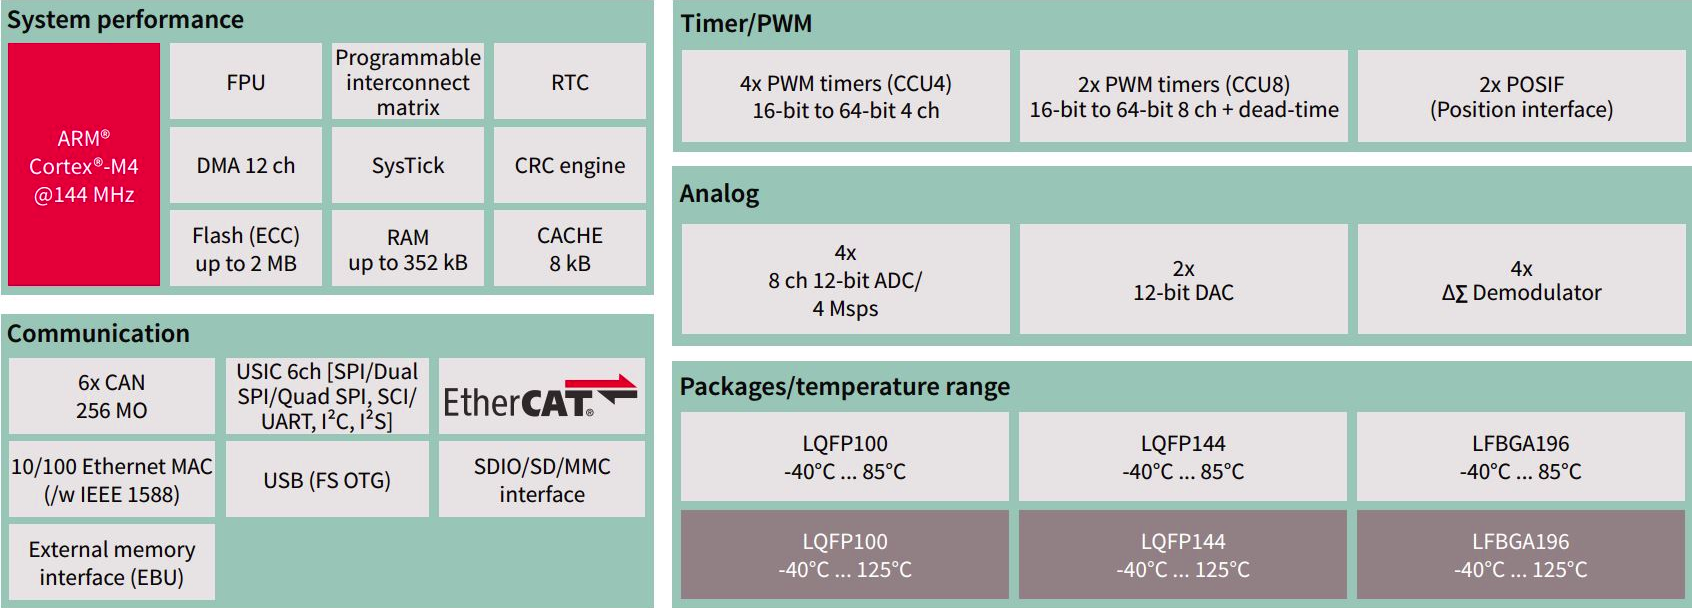
\includegraphics[scale=.2]{img/cap3/xmc4800_data}
  \caption{Carácteristicas del microcontrolador XMC4800. MO: Message Objects, Msps: Mega samples per second.}
  \label{cap3_xmc4800_data}
\end{figure}

La configuración de perifiericos en este tipo de microcontroladores suele ser una tarea compleja, dada las distintos \textit{pin out} y configuraciones de cada uno. Afortunadamente, el fabricante provee un IDE llamado Dave (Digital Application Virtual Engineer) que posee herramientas de generación de código a partir de una interfaz gráfica.

Otra carácteristica importante es que la placa de desarrollo escogida de este microcontrolador, la XMC4800 Relax EtherCAT Kit (Figura \ref{cap3_xmc4800}), posee la mayoría de componentes externos necesarios para el uso de las distintas funcionalidades del microcontrolador, como dos Ethernet PHY (transceiver) para la comunicación EtherCAT. Además integra un programador y debugger Segger J-Link que permite establecer \textit{break points} en el código y acceder a distintos registros de microcontrolador en tiempo real.

\begin{figure}[ht]
  \centering
  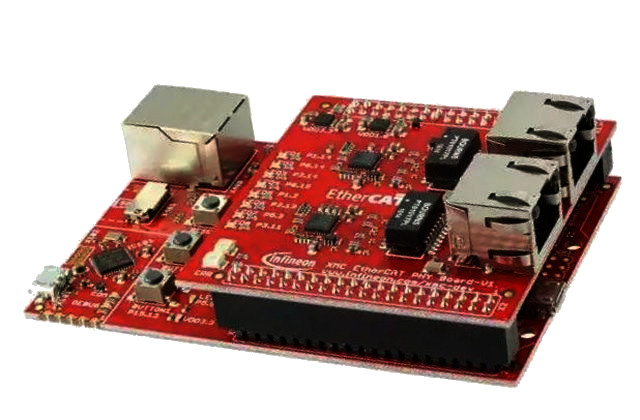
\includegraphics[scale=.4]{img/cap3/xmc4800}
  \caption{Placa de desarrollo XMC4800 Relax EtherCAT Kit.}
  \label{cap3_xmc4800}
\end{figure}
 

\subsection{Puente H}

Para la etapa de potencia se selecciono un puente H basado en el IC BTN8982TA, el cual corresponde a un \textit{half bridge} de alta corriente para aplicaciones con motores, contiene 
un MOSFET canal P para el \textit{high-side} y un canal N para el \textit{low-side}, ambos con un driver integrado, que permite su disparo directo desde un microcontrolador.

Para implementación se uso la placa de desarrollo \textit{Motor Control Shield}, que usa dos BTN8982TA en una configuración \textit{full bridge}, una imagen referencial se muestra  en la Figura \ref{cap2_punteh_infineon}, las principales carácteristicas:

\begin{itemize}
\item Control bidireccional de motor DC con escobillas de hasta \SI{250}{\watt} continuos.
\item Rango de tensión de entrada nominal \SI{8}{\volt} a \SI{18}{\volt} (\SI{6}{\volt} a \SI{40}{\volt} máximo).
\item Corriente máxima \SI{30}{\ampere}, restringida por la disipación del PCB (BTN8982TA tiene un limite de \SI{55}{\ampere}).
\item Frecuencia de conmutación hasta \SI{30}{\kilo\hertz}.
\end{itemize}

\begin{figure}[ht]
  \centering
  \includegraphics[scale=.35]{img/cap2/puenteh_infineon}
  \caption{Puente H fabricado por Infineon Technologies AG\textregistered \, basado en BTN8982TA.}
  \label{cap2_punteh_infineon}
\end{figure}

\subsection{Sensor de corriente}

Para la etapa de control del motor del motor de corriente continua es necesario contar con un sensor de corriente. Existen diversas tecnologías y técnicas de medición de corriente disponibles.

En el desarrollo de este trabajo se consideró el uso de un sensor de efecto hall Infineon TLI4970, su principal característica corresponde a la integración del ADC, DSP y acondicionamiento de señal se encuentran dentro del mismo \textit{package} \cite{infineonTLI4970}. Esto reduce la cantidad de elementos externos necesarios para realizar la medición de corriente. La Figura \ref{cap3_tli4970}, muestra el diagrama de bloques de los elementos internos del sensor.

\begin{figure}[H]
  \centering
  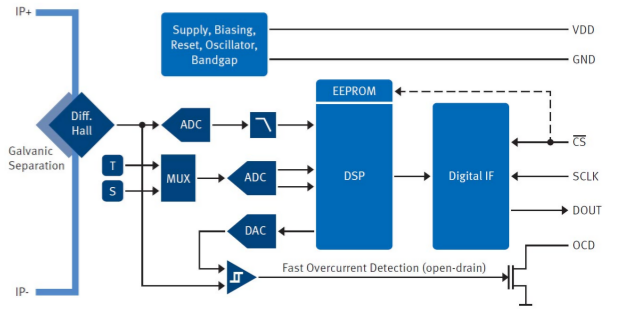
\includegraphics[scale=.45]{img/cap3/tli4970}
  \caption{Diagrama del sensor de corriente TLI4970.}
  \label{cap3_tli4970}
\end{figure}

El sensor tiene un rango máximo \SI{\pm 25}{\ampere} y una resolución de 10 bits. La salida del sensor se obtiene usando el protocolo SPI conectado directamente al microcontrolador.

\subsection{Estimación de velocidad}

El robot Scorbot cuenta con \textit{encoders} en cada uno de los motores que accionan sus articulaciones.

Estimación esta sujeta a errores de cuantización

Para lograr mejores resultados es conventiente usar un estimador de velocidad, el cual realiza seguimiento de la velocidad considerando la medidas obtenidas del encoder sin utilizar una diferenciación de forma explicita. Consideremos un estimador de velocidad basado en un \textit{loop} PI, donde las estimaciones de la posición $\hat{x}$ y velocidad $\hat{v}$ estan dadas por:

\begin{eqnarray}
\hat{x} &=& \frac{1}{s} \hat{v} \\
\hat{v} &=& \left( \frac{k_i}{s} + k_p \right) (x-\hat{x})
\end{eqnarray}

Luego de una manipulación algebraica se puede obtener la siguiente expresión para $\hat{x}$.

\begin{equation}
\hat{x} = \frac{1+s\frac{k_p}{k_i}}{1+s\frac{k_p}{k_i}+s^2\frac{1}{k_i}}x
\end{equation}

A partir de expresión anterior podemos expresar el error de estimación:

\begin{eqnarray}
\tilde{x} &=& x - \hat{x} \\
\tilde{x} &=& x \left(1 -  \frac{1+s\frac{k_p}{k_i}}{1+s\frac{k_p}{k_i}+s^2\frac{1}{k_i}} \right) \\
\tilde{x} &=& x \left(\frac{s^2 \frac{1}{k_i}}{1+s\frac{k_p}{k_i}+s^2\frac{1}{k_i}}\right)
\end{eqnarray}

De la última expresión, usando el teorema del valor final, podemos obtener que la estimación tendrá cero error en estacionario para entradas de tipo escalón y rampa. La dinámica del estimador esta dado por los polos $p_i$ de la función de tranferencia, para este caso consideremos un ancho de banda deseado $B$ y un coeficiente de amotiguamiento $\zeta=1$ (criticamente amortiguado). De esta forma la ecuación carácteristica esta dada por:

\begin{equation}
p_i = -\frac{k_p}{2} \pm \sqrt{k_p^2-4k_i}
\end{equation}

La restricción de amortiguamiento critico hace que los polos sean reales y únicos, por que se obtiene:

\begin{eqnarray}
k_p &=& 2 B \\
k_i &=& \frac{kp^2}{4}
\end{eqnarray}

La Figura \ref{cap3_estimador_vel} muestra el diagrama de bloques del estimador de velocidad. Notar que la función de transferencia corresponde a un sistema lineal, por lo que puede en un microcontrolador usando los metodos de discretización descritos anteriormente.

\begin{figure}[H]
  \centering
  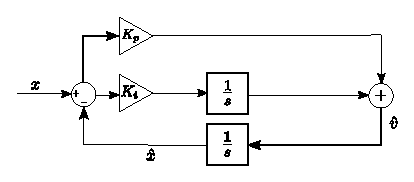
\includegraphics[width=0.8\textwidth]{img/cap3/estimador}
  \caption{\textit{Tracking loop} para estimación de velocidad.}
  \label{cap3_estimador_vel}
\end{figure}


\section{Integración de hardware}

Con el fin de reducir el tiempo de desarrollo, se consideró el uso de placas de desarrollo que provee el fabricante, de esta forma se usaron directamente el kit del microcontrolador XMC4800 y el puente H basado en el BTN8982TA. Para lograr una integración de hardware modular se consideró  el diseño de una PCB que permita el montaje de los kits y otros componentes usados.

El diseño del PCB contempló la interconexión del puente H, el microcontrolador y el sensor de corriente TLI4970. La PCB debe considerar los siguientes aspectos:
\begin{itemize}
\item Entregar la alimentación necesaria a cada dispositivo, esto el voltage y una capacidad de corriente adecuada.
\item Ajuste de nivel de voltaje para los elementos lógicos, como switches y encoders.
\item Uso de conectores de potencia y control adecuados para la aplicación.
\end{itemize}



